We validate our approaches on several image datasets.  The evaluation are mainly based on qualitative and qualitative results. For the qualitative evaluation, we examine the quality of the samples generated from our models (fixing one block while sampling from another), we do data exploration of learned representations using clustering plots, and we also analyze the correlation matrix learned by our methods. In terms of quantitative results, we provide the classification accuracy for the prediction task using learned latent representations. Results and discussions are provided in later sections.

\subsection{Setup}
\paragraph{Data} We evaluate our methods on $3$ image datasets: MNIST dataset~\footnote{http://yann.lecun.com/exdb/mnist/}, Face dataset~\footnote{http://www.multipie.org/} and Norb dataset~\footnote{http://www.cs.nyu.edu/~ylclab/data/norb-v1.0/}. MNIST contains $50,000$ training and $10,000$ testing samples from 10 different digit classes, and each image mainly contains two factors of variation: digit class and writing style. The face dataset contains the human face images from $68$ identities with different lighting conditions and views, which in total provides $3$ different factors\footnote{We use only subset of the original dataset.}. The Norb dataset also contains 3 factors including category, orientation and brightness\footnote{In fact, the Norb dataset contains more than 3 factors such as category, subcategory.etc. But in this experiments, we manually merge some of the factors which gives us total 3 factors in the end}.

\paragraph{Details} For each dataset, we convert the feature vector into normal distribution with mean zero and unit variance. We evaluate the performance on several models which are the combinations of different prior and variational posterior distributions. The summary of the proposed models and baseline model are shown in Table~\ref{table:model}

The model A is the baseline from \cite{kingma2013auto}, which assumes $\mathcal{N}(0,1)$ prior on $p(\mathbf{z})$ and Gaussian distribution with diagonal covariance $\mathcal{N}(\mu, \sigma^2\mathbf{I})$ for variational posterior distribution $q_{\phi}(\mathbf{z}|\mathbf{x})$

The model B and C are the ones trained with known block structure (i.e the number of blocks, and the size of each block). We put Gaussian distribution with block diagonal covariance $\mathcal{N}(\mu, \Lambda)$ on $p(\mathbf{z})$, where we explicitly parameterize $\Lambda$ with $L$ sub-blocks whose size are known. The main difference between model B and model C is that we use different forms of covariance to parameterize the variational posterior distribution $q_{\phi}(\mathbf{z}|\mathbf{x})$. For model B, we use Gaussian distribution with diagonal covariance $\mathcal{N}(0,\sigma^2\mathbf{I})$. On the other hand, for model C, we parameterize it using block diagonal covariance, where each sub-block is generated from MLP.

The model D is the generalization of model B and C to the case that the block structure is unknown. Instead of putting explicitly defined covariance on prior $p(\mathbf{z})$, instead, we put variable clustering prior~\cite{palla2012nonparametric} which introduces cluster membership for each dimension of latent representation.


\begin{table}
\centering
\begin{tabular}{|l|c|c|c|}
\hline
\backslashbox{Posterior}{Prior}  & $\mathcal{N}(0,1)$ & BLK & BLK(unknown) \\
\hline
 Diagonal& Model A & Model B & Model D\\
 \hline
 BLK &  & Model C& \\
% & all & all\\
\hline
\end{tabular}
\caption{The summary of the models evaluated in this paper}
\label{table:model}
\end{table}


\subsection{MNIST datset}
\paragraph{Learning with $4$ hidden units and $2$ blocks}
We assume the size of hidden units is $4$, and the input data has two factors of variation. For model B and C, we define the covariance matrix having two $2$ by $2$ sub-blocks on the diagonal. This enforces that the first two hidden units control one factor, and the remaining two control the second factor, but we don't define which factor controls digit class or writing style before learning the model. For model A, since we don't explicitly define the grouping structures of hidden units, we need to do greedy search to figure out the group of hidden units control each of the factors. On the other hand, model D can automatically discover the group of hidden units without defining the structure. This brings one significant benefit in the cases that some factors contain much more information than others, and we expect that model D is able to assign more hidden units to those complex factors and less to the simpler ones. We will demonstrate some interesting observations in later section.

\paragraph{Quality of samples from different models}
\begin{figure}
\centering
    \begin{subfigure}[b]{0.9\textwidth}
    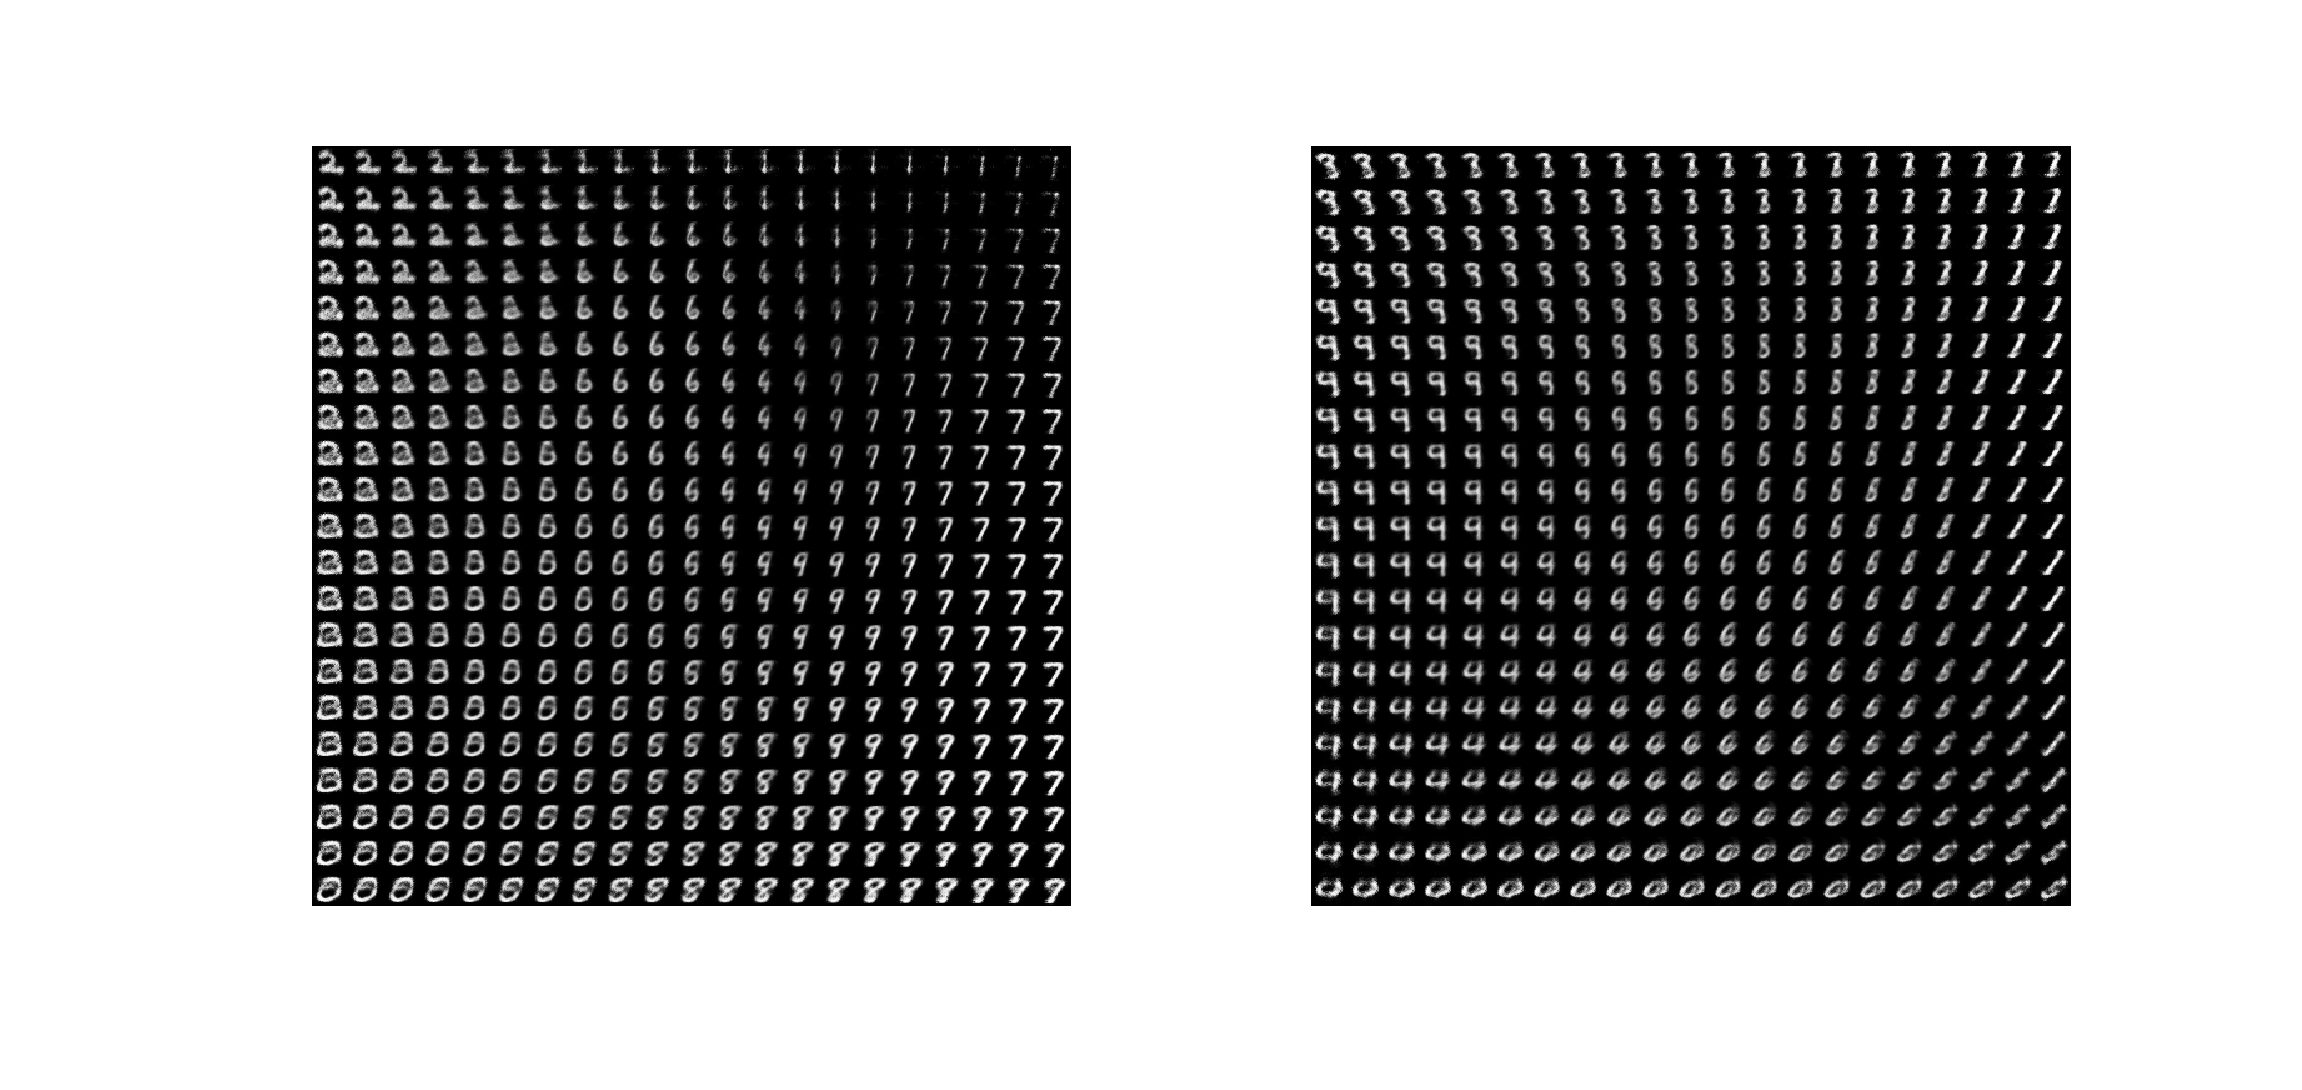
\includegraphics[width=\textwidth]{images/sampleWelling.eps}
    \vspace{-3\baselineskip}
    \caption{Model A}
    \label{fig:us-air}
    \end{subfigure}
	\begin{subfigure}[b]{0.9\textwidth}
    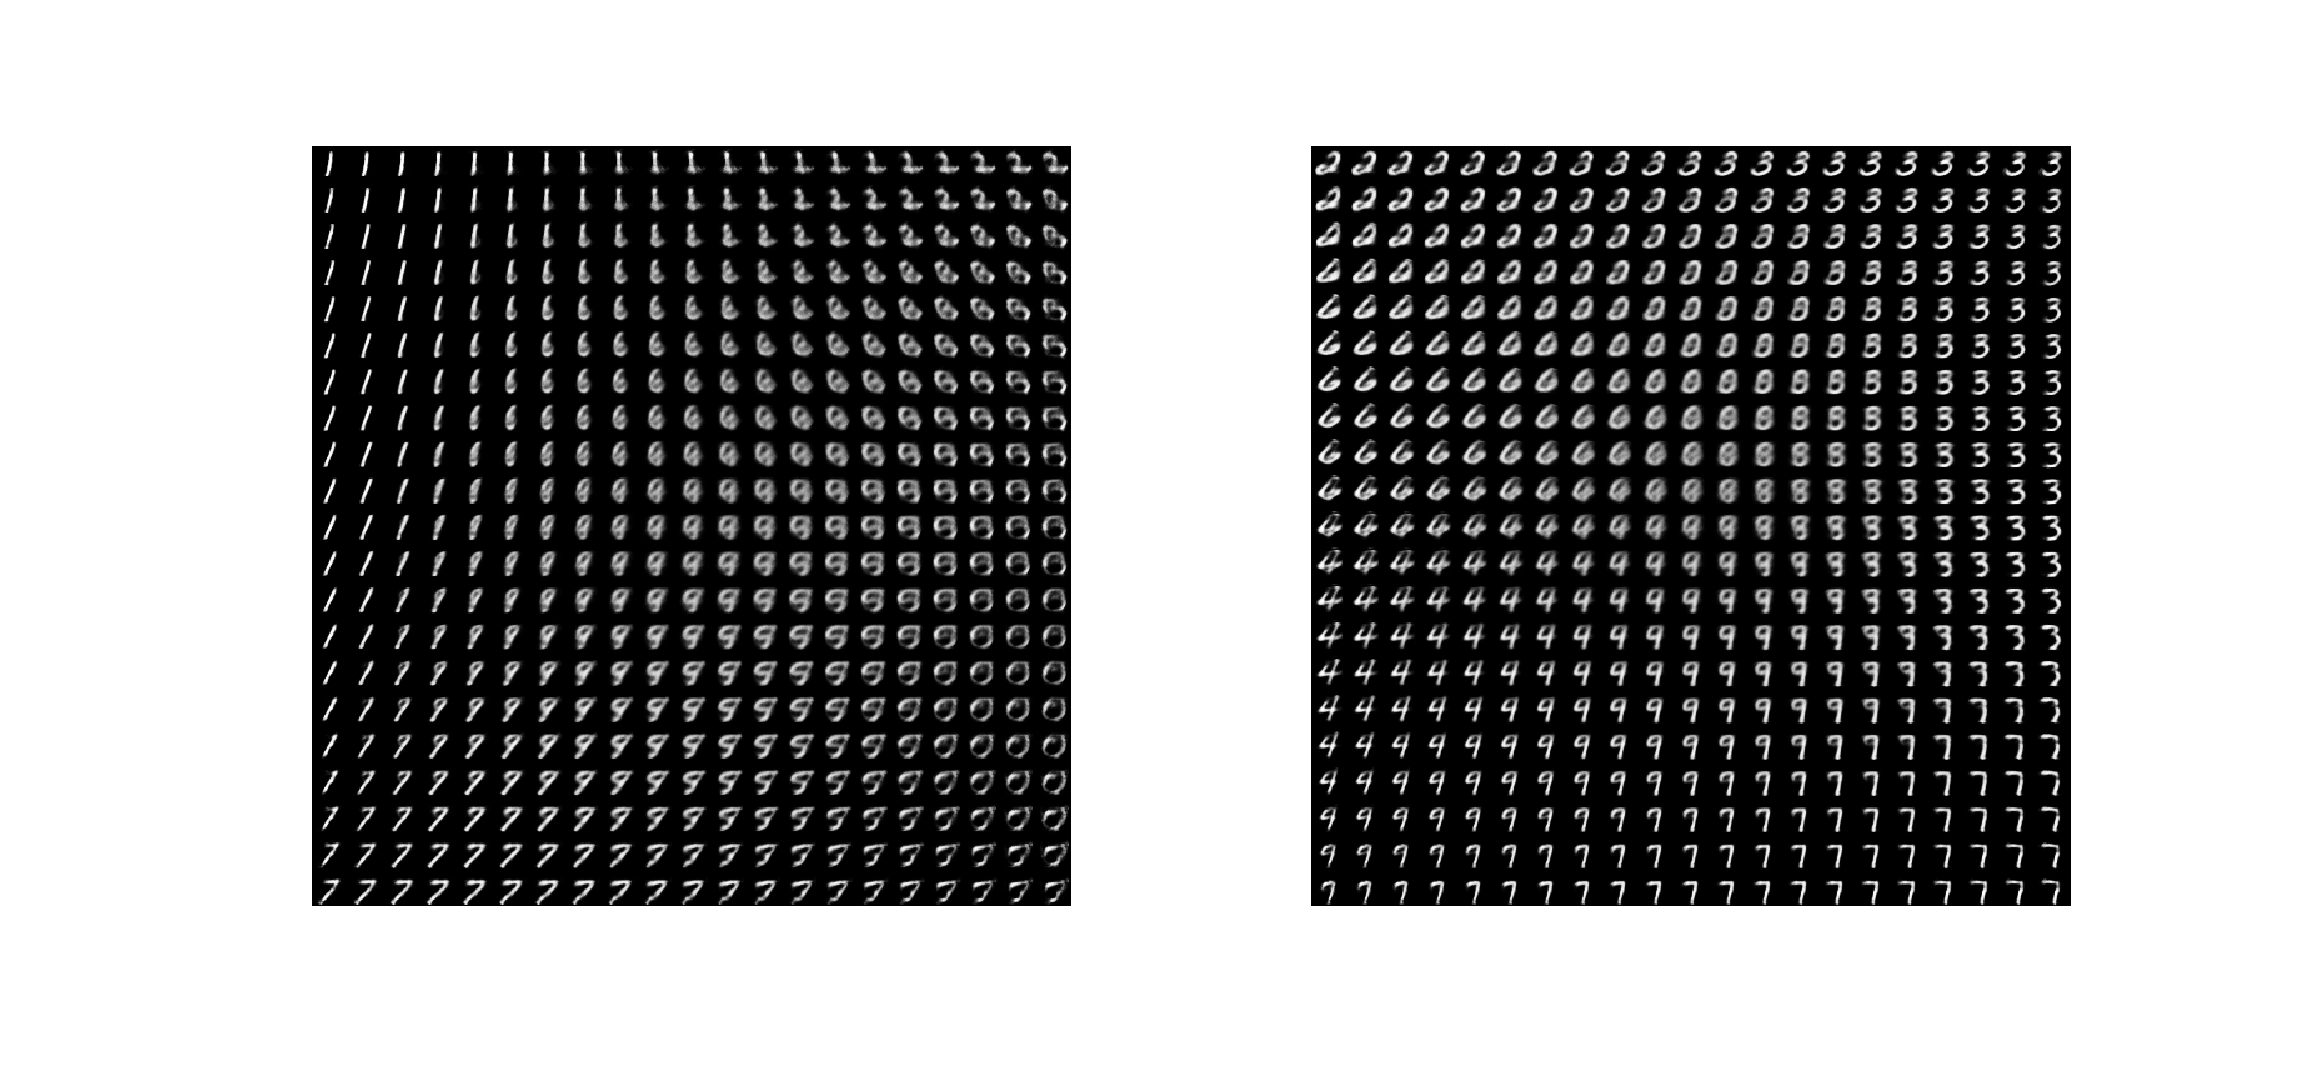
\includegraphics[width=\textwidth]{images/sampleNWdiag.eps}
    \vspace{-3\baselineskip}
    \caption{Model B}
    \label{fig:us-air}
    \end{subfigure}
    \begin{subfigure}[b]{0.9\textwidth}
    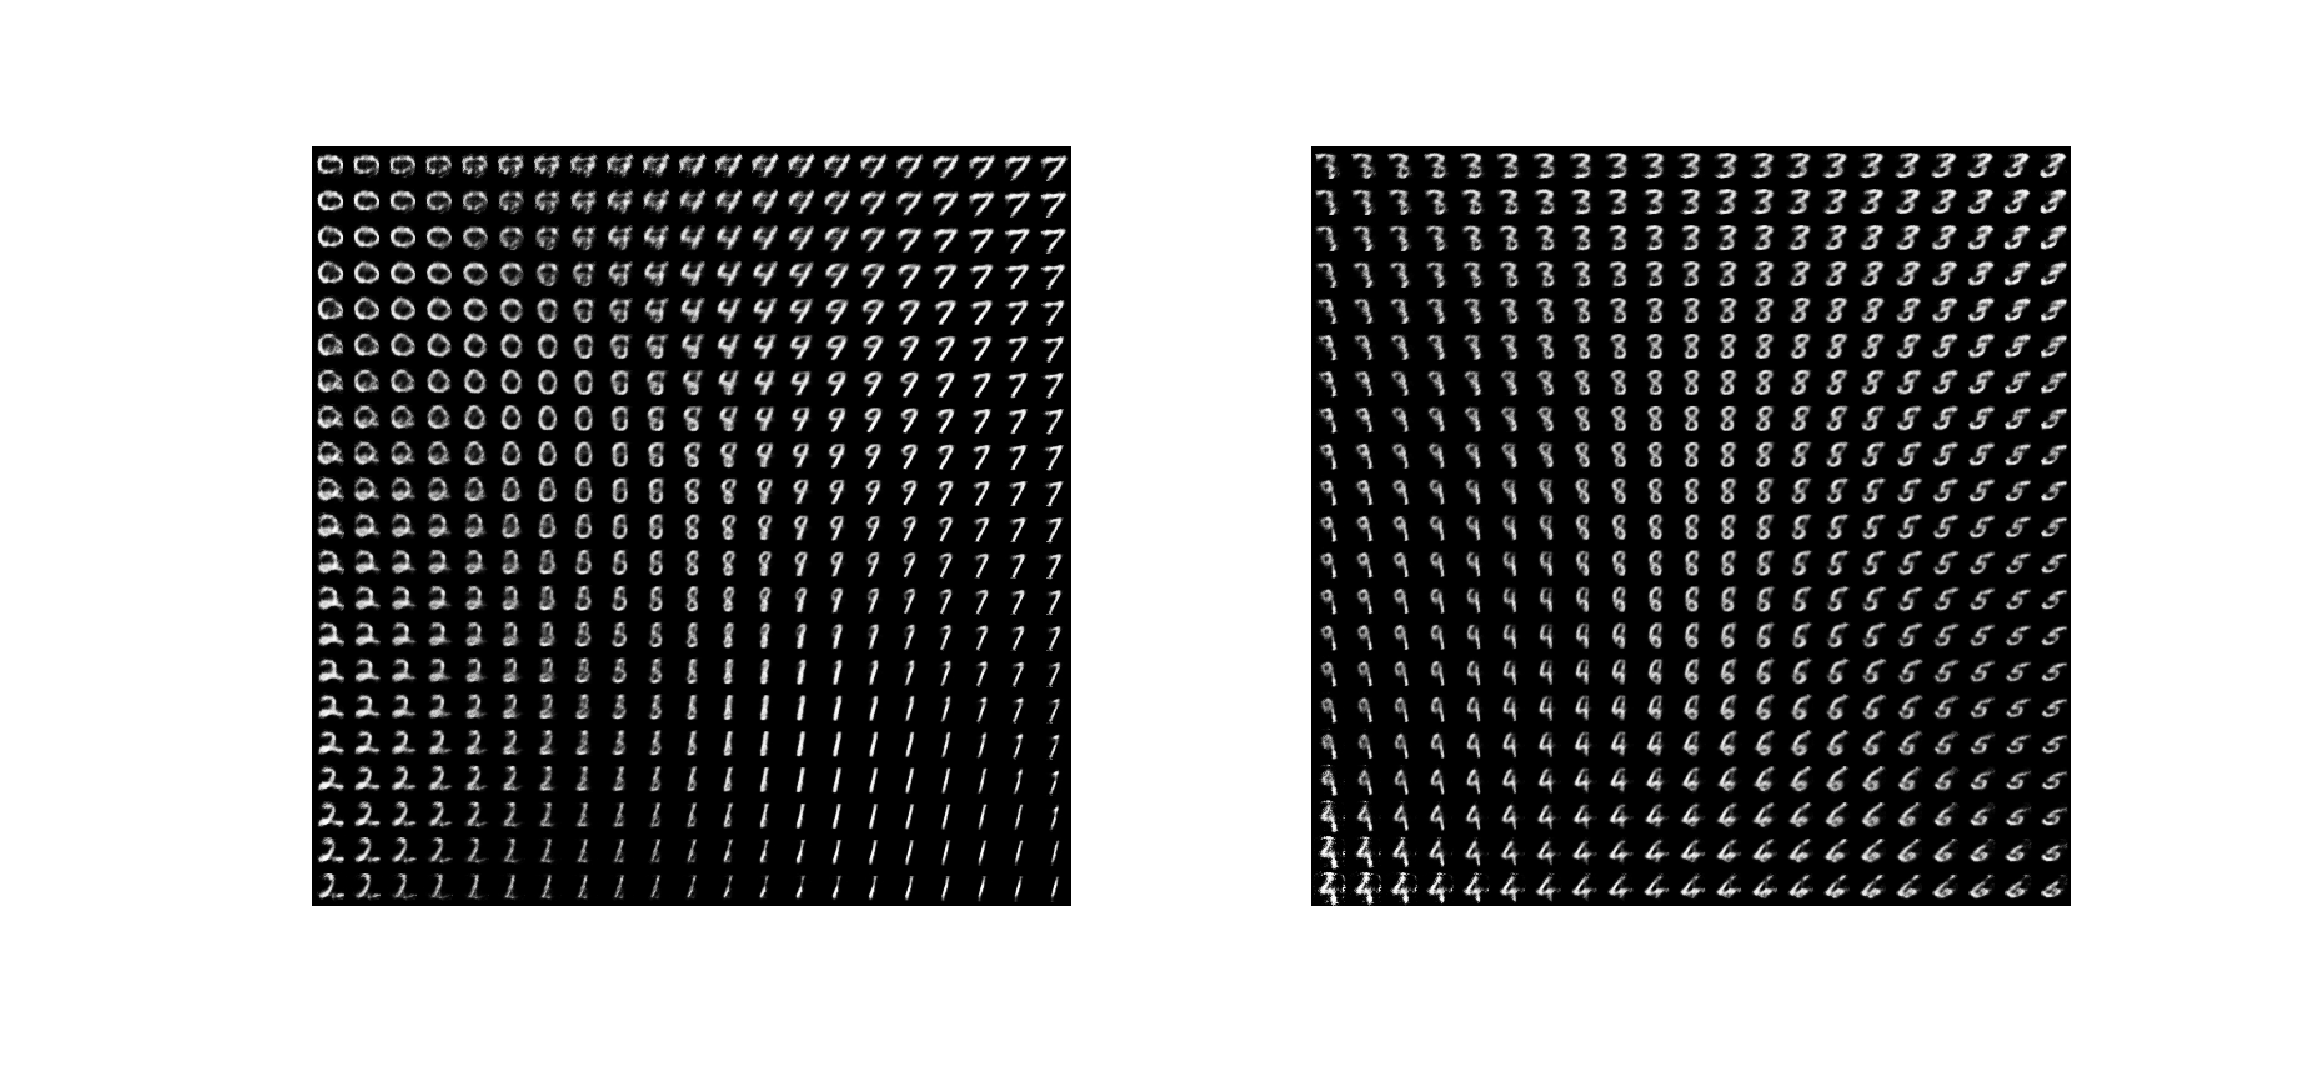
\includegraphics[width=\textwidth]{images/sampleNWblock.eps}
    \vspace{-3\baselineskip}
    \caption{Model C}
    \label{fig:us-air}
    \end{subfigure}
    \begin{subfigure}[b]{0.9\textwidth}
    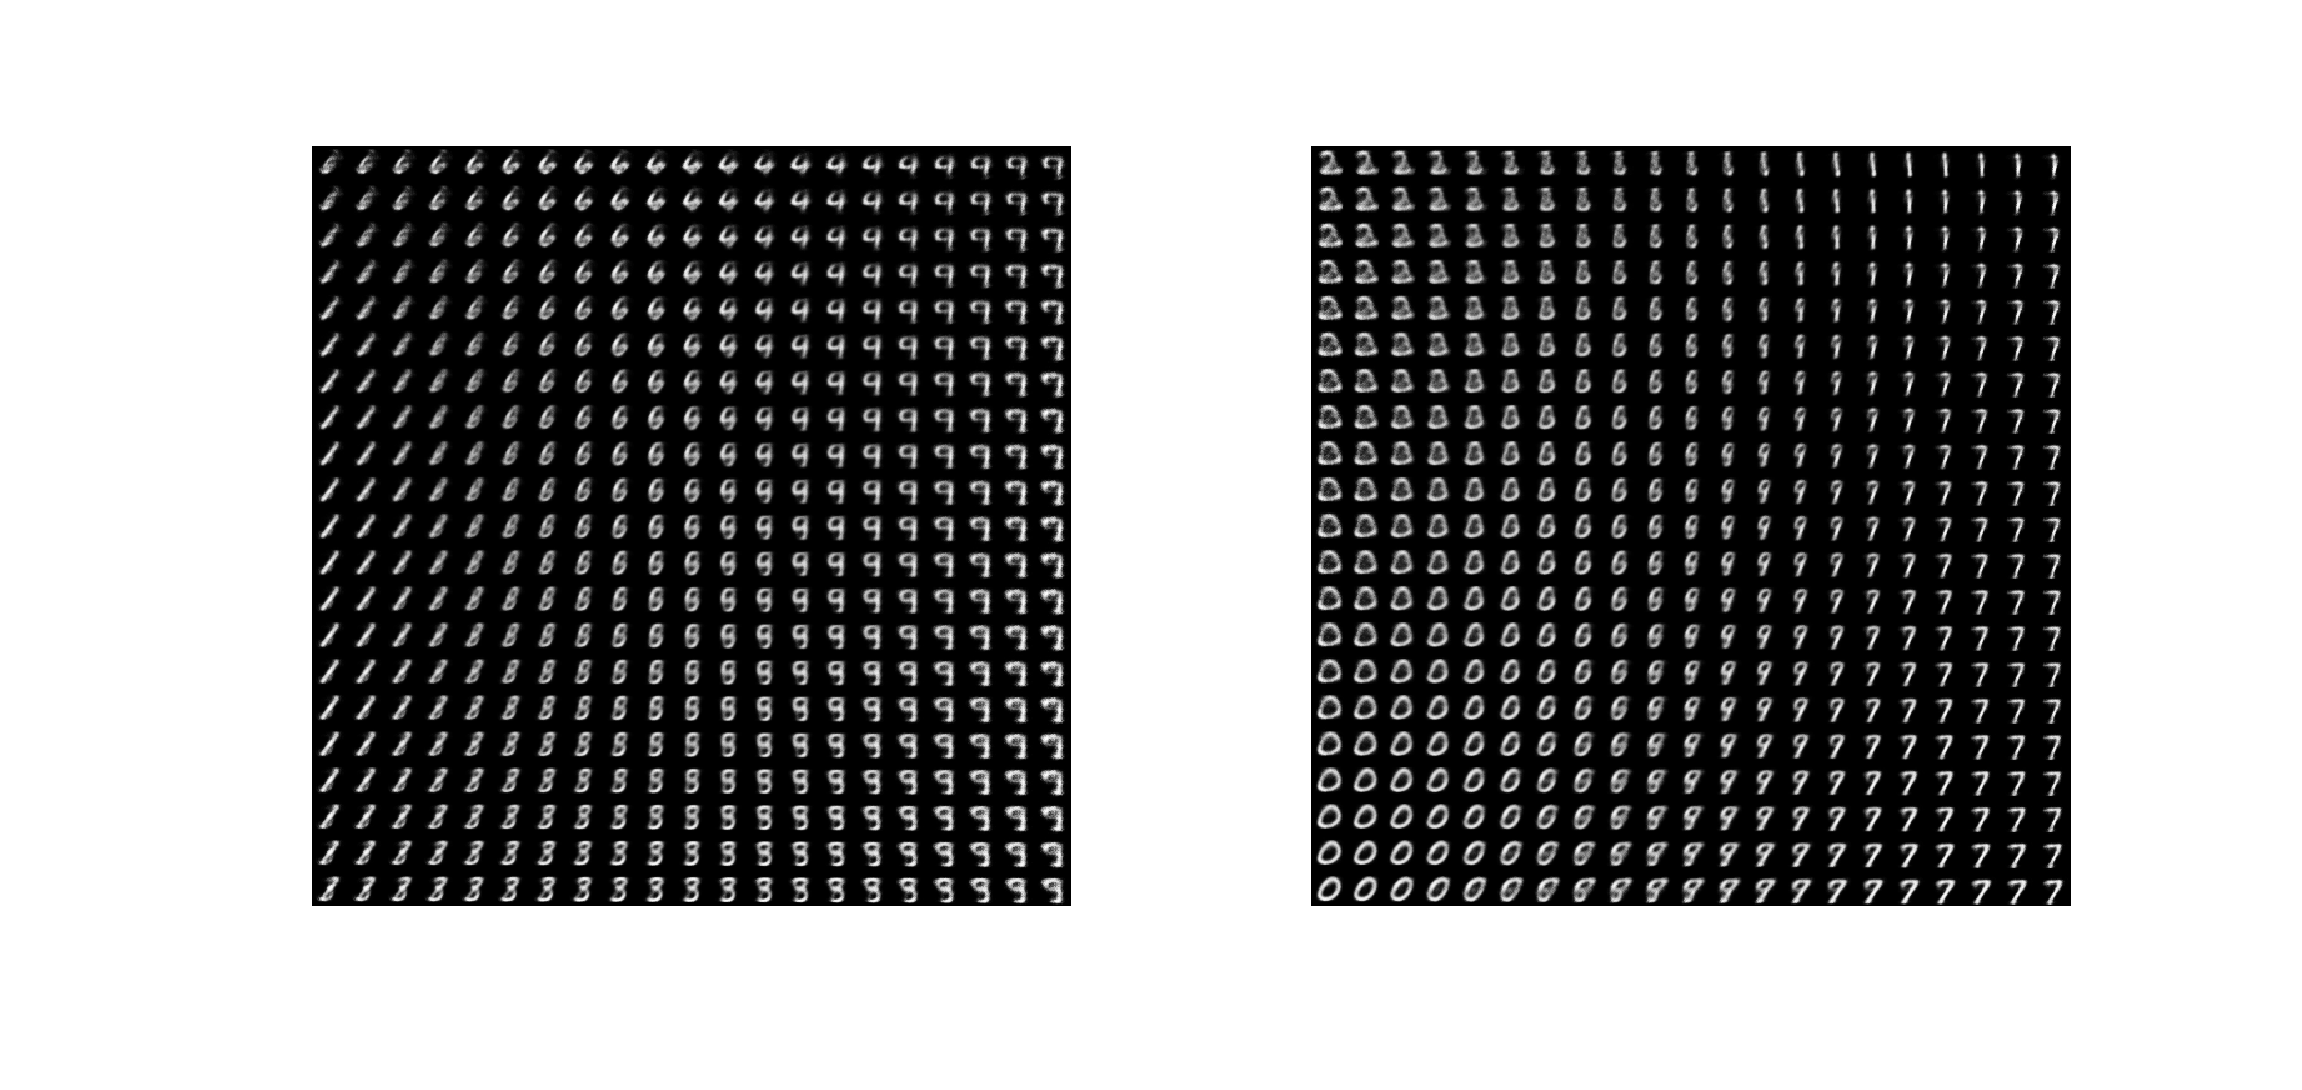
\includegraphics[width=\textwidth]{images/sampleAverage.eps}
    \vspace{-3\baselineskip}
    \caption{Model D}
    \label{fig:us-air}
    \end{subfigure}
    \caption{Generated samples from each model on MNIST dataset. The left figure shows the samples by fixing the first block (mean sample), and sample for the second block. Similar analogy applies to the right figure.}\label{fig:animals}
    \label{fig:MNISTsamples}
\end{figure}

Figure~\ref{fig:MNISTsamples} shows the generated samples from different models. The samples are generated by fixing one block and sample on another. By fixing we mean that we use the "mean" sample. In order to cover the sample space more broadly, we divide the space into grids and uniformly sample within that grid. The figure shows some interesting observations in terms of change of digit class and writing style. For model A, we could easily see that the digit class and writing style mixed together. The model B, although it's a bit better than model A, it's still hard to see the dominant factors for each block. However, for model C and D, the different is more distinguishable. The writing style factor dominates in the right figure of model C, and left figure of model D. And the remaining figures denote the change of digit classes. Please note that for this dataset, model D learns to assign two hidden units to one factor, and the other two for another factor.

\vspace{-0.1cm}
\paragraph{Predictive accuracy on the learned representations}
We also evaluate the predicative performance on the learned representation $\mathbf{z}$. For this purpose, we run the multinomial logistic regression on each block, and record the maximum accuracy. We expect that the factor encodes the digit class gives better prediction accuracy. Table~\ref{tab:regression} shows the classification results on MNIST dataset. The notation MNIST($4d_{\text{factor}}$) means that the classification accuracy is computed using one factor from the model that trained with $4$ hidden units, and MNIST($4d_{\text{all}}$) means that the result is computed using all the hidden units.

\begin{table*}[htb]
	\begin{center}
		\begin{small}
			\begin{sc}
				\begin{tabular}{lcc}
					\hline
					Data set & MNIST(4D\_factor) & MNIST(4D\_all)  \\
					\hline
					Model A& 53.9  & 74.6\\
					Model B &44.4 & 77.4\\
					Model C & 56.7 &80.5\\
					Model D & 48.2 & 71.6\\
					\hline
					% & all & all\\
				\end{tabular}
			\end{sc}
		\end{small}
        \vspace{0.2cm}
		\caption{Predictive performance on the hidden representation which encodes the digit class factor}
\vspace{-0.5cm}		
\label{tab:regression}
	\end{center}
\end{table*}

The difference between these models is not obvious. In general, the model with block diagonal prior and block diagonal variational posterior performs best. This is reasonable since we explicitly define the block structure which is equivalent to putting hard constraints. Although the model D does give least accuracy when we using all the hidden units, the performance on the digit factor is reasonablely good. The baseline model A gives the best accuracy when we only consider the digit factor. But please note that this factor is found by greedy search which provides the best accuracy, which might be unfair for comparisons with other models. 

\subsection{Face dataset}
Face dataset contains $3$ factors. However, the image is more complicated than MNIST dataset, which means that each image contains more information. Thus, for this experiment, we increase the number of hidden units to $6$. Figure~\ref{fig:FacesamplesModel3} shows the generated samples from model C. We set the size of each factor having $2$ hidden units. From this figure, we can easily see that block 1 encodes identity, block 2 encodes brightness and block 3 encodes view factor.

More interesting experiments are for model D. Figure~\ref{fig:Facesamples} shows the generated samples from model D by sampling from one block while fixing others (with mean sample). From the figure, we can easily see that the block 1 controls the lighting condition, block 2 controls identity and block 3 controls different views. Figure 5 shows the correlation matrix on the learned representations. Between these two figures, the right one clearly has block diagonal covariance structure, while the correlation for the left one almost has diagonal structure.

This right figure clearly shows the block structure of each factor for model D. In our case, the model assigns one hidden unit to block 1, and four hidden units to block 2, and the remaining one hidden unit to block 3. This is an interesting observation but is quite reasonable, since the there is much more information is contained in the identity factor. In order to encode more complex information, our model naturally provides more hidden units to it. This provides significant benefits over other models.
\begin{figure}
\centering
    \begin{subfigure}[b]{0.5\textwidth}
    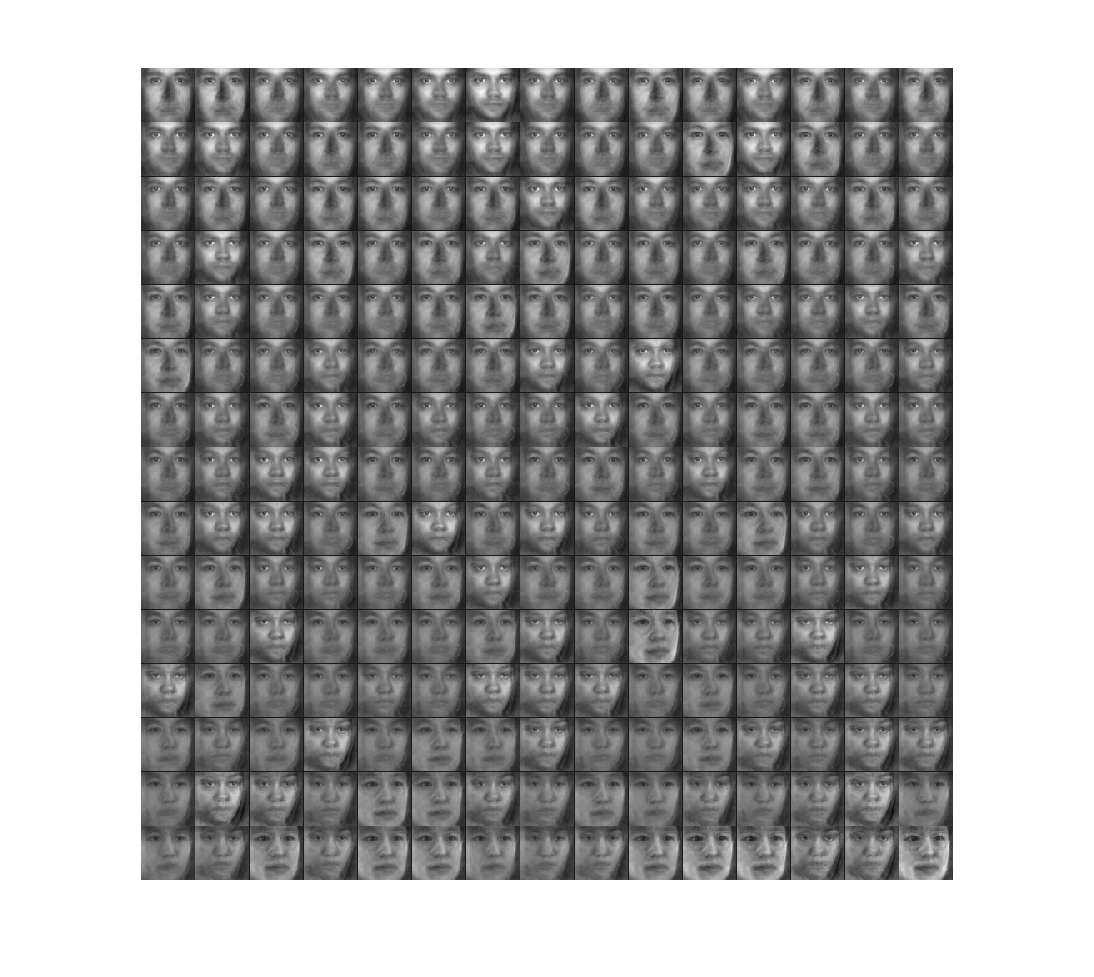
\includegraphics[width=\textwidth]{images/faceNWblock1.eps}
    \vspace{-2\baselineskip}
    \caption{Block 1 (2 hidden unit)}
    \end{subfigure}
	\begin{subfigure}[b]{0.5\textwidth}
    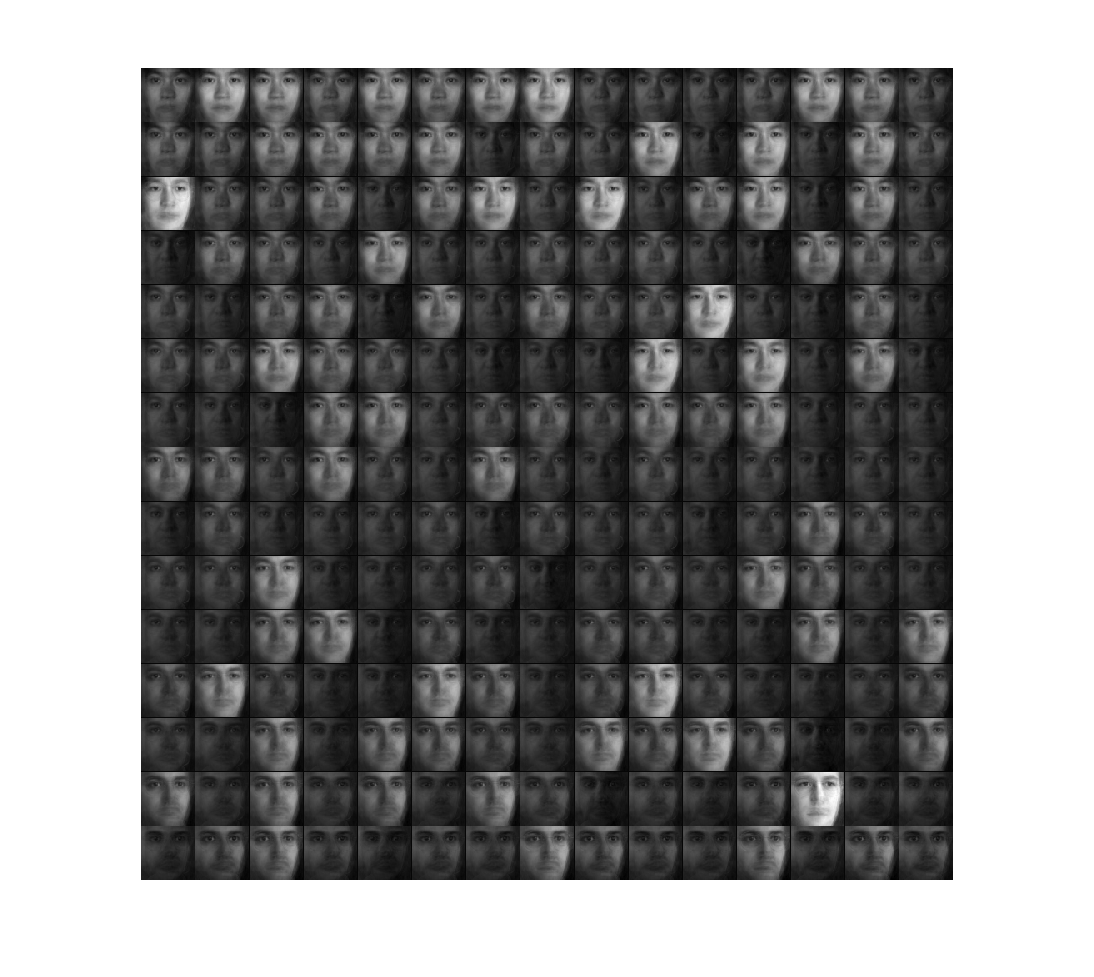
\includegraphics[width=\textwidth]{images/faceNWblock2.eps}
    \vspace{-2\baselineskip}
    \caption{Block 2 (2 hidden units)}
    \end{subfigure}
    \begin{subfigure}[b]{0.5\textwidth}
    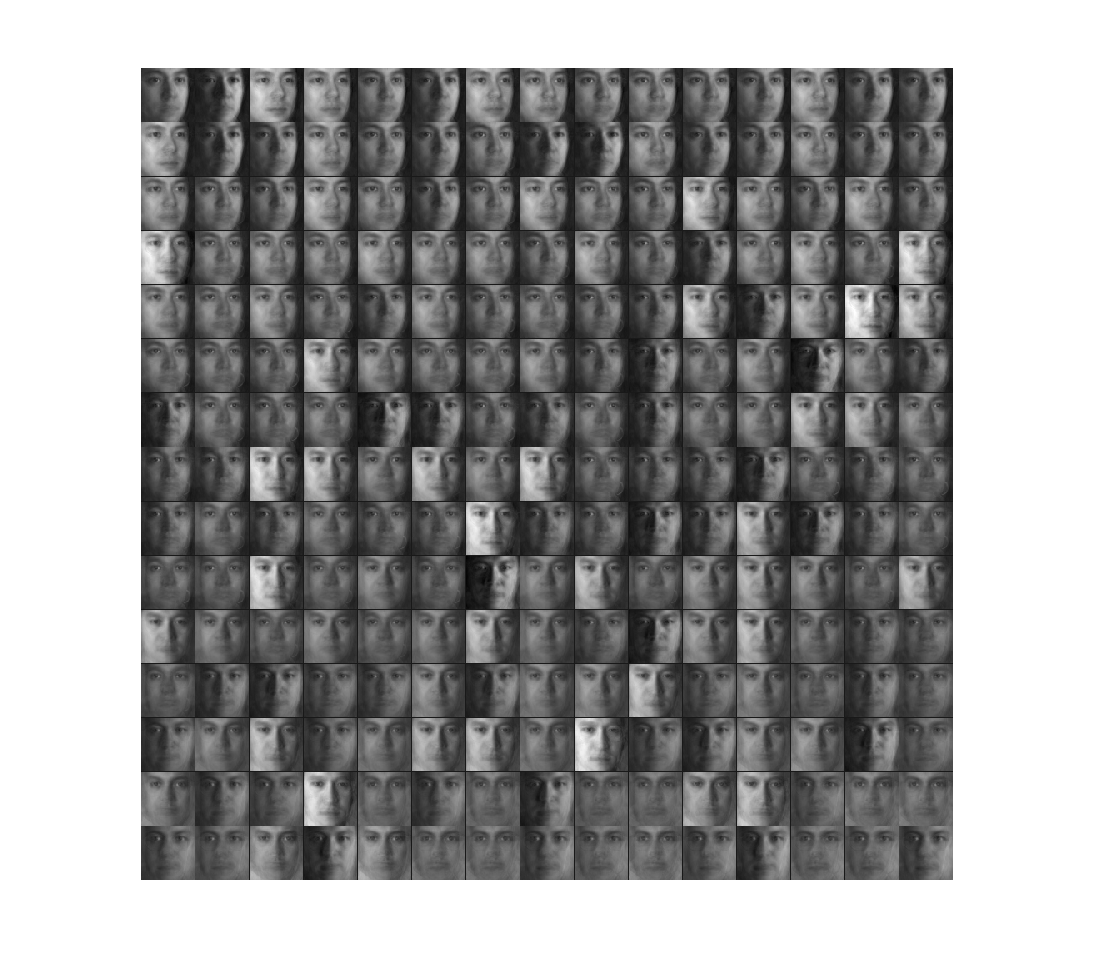
\includegraphics[width=\textwidth]{images/faceNWblock3.eps}
    \vspace{-2\baselineskip}
    \caption{Block 3 (2 hidden unit)}
    \end{subfigure}
    \caption{Generated face samples from \textbf{model C}. Block 1 means that we sample for block 1 and fixed others (with mean), and etc.}\label{fig:animals}
    \label{fig:FacesamplesModel3}
\end{figure}



\begin{figure}
\centering
    \begin{subfigure}[b]{0.5\textwidth}
    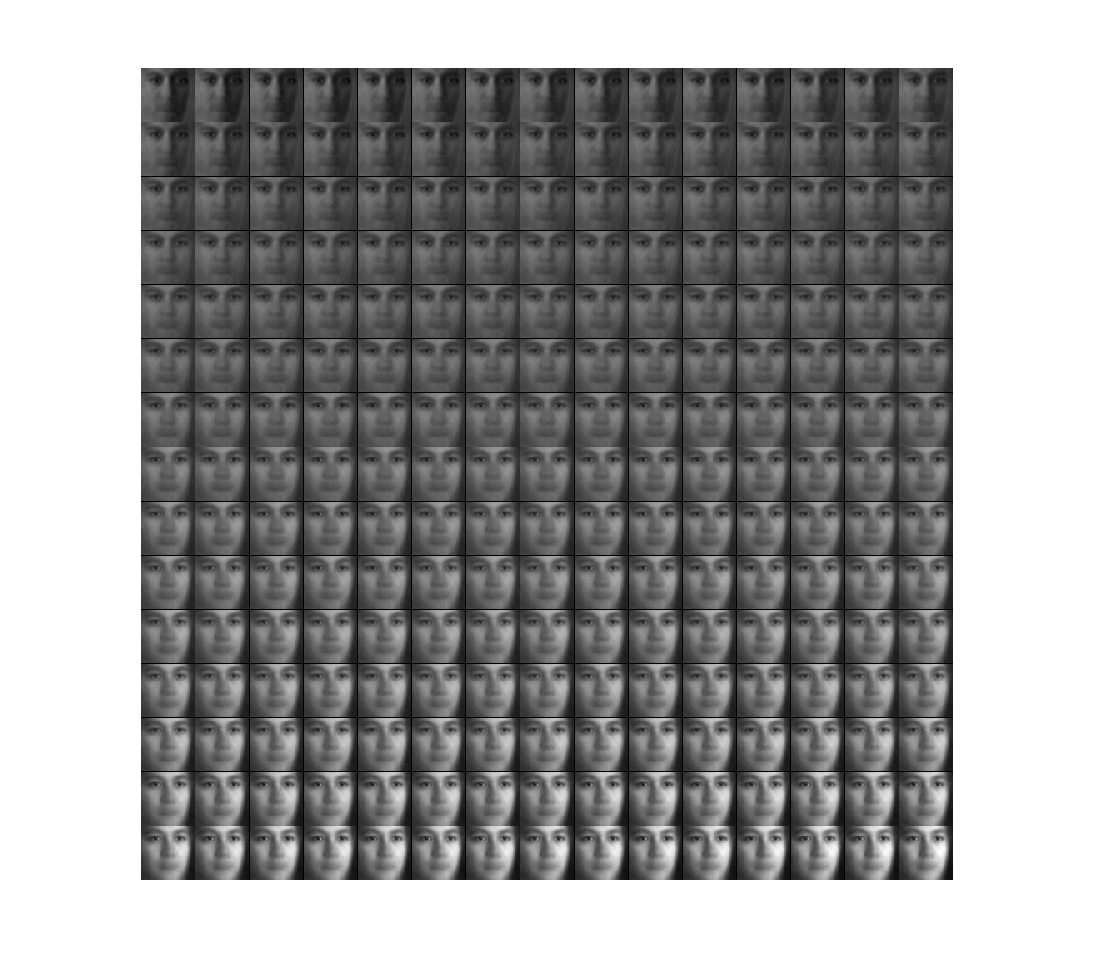
\includegraphics[width=\textwidth]{images/faceBlock1.eps}
    \vspace{-2\baselineskip}
    \caption{Block 1 (1 hidden unit)}
    \end{subfigure}
	\begin{subfigure}[b]{0.5\textwidth}
    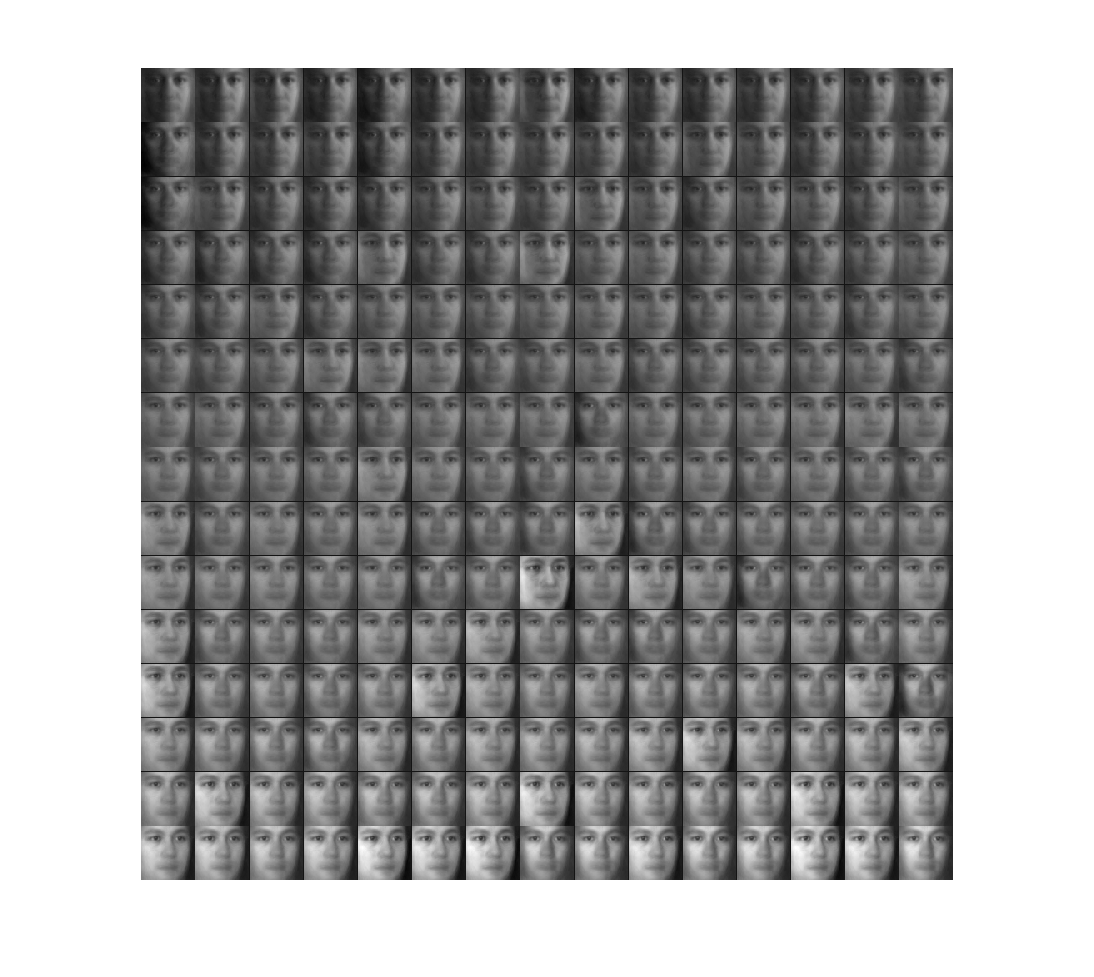
\includegraphics[width=\textwidth]{images/faceBlock2.eps}
    \vspace{-2\baselineskip}
    \caption{Block 2 (4 hidden units)}
    \end{subfigure}
    \begin{subfigure}[b]{0.5\textwidth}
    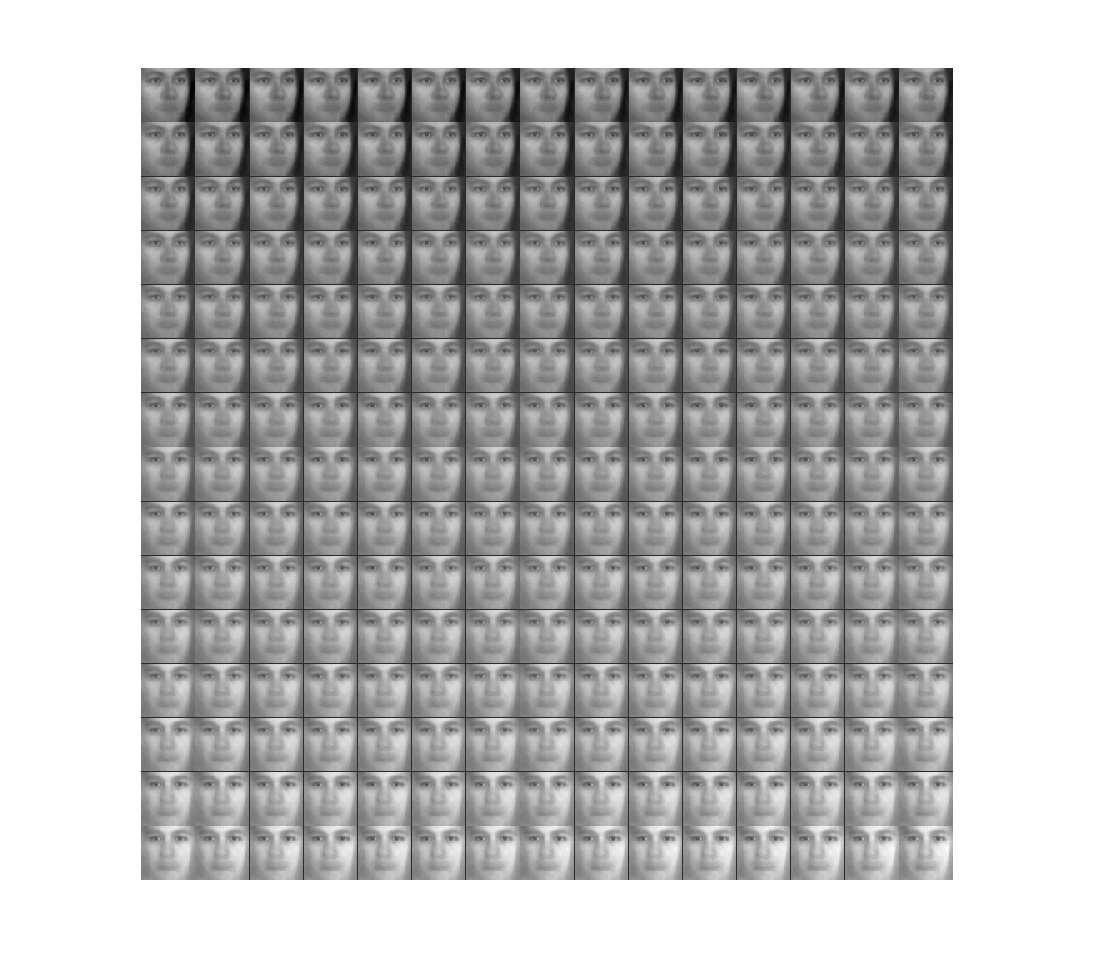
\includegraphics[width=\textwidth]{images/faceBlock3.eps}
    \vspace{-2\baselineskip}
    \caption{Block 3 (1 hidden unit)}
    \end{subfigure}
    \caption{Generated face samples from \textbf{model D}. Block 1 means that we sample for block 1 and fixed others (with mean), and so on}\label{fig:animals}
    \label{fig:Facesamples}
\end{figure}


\begin{figure}
\centering
    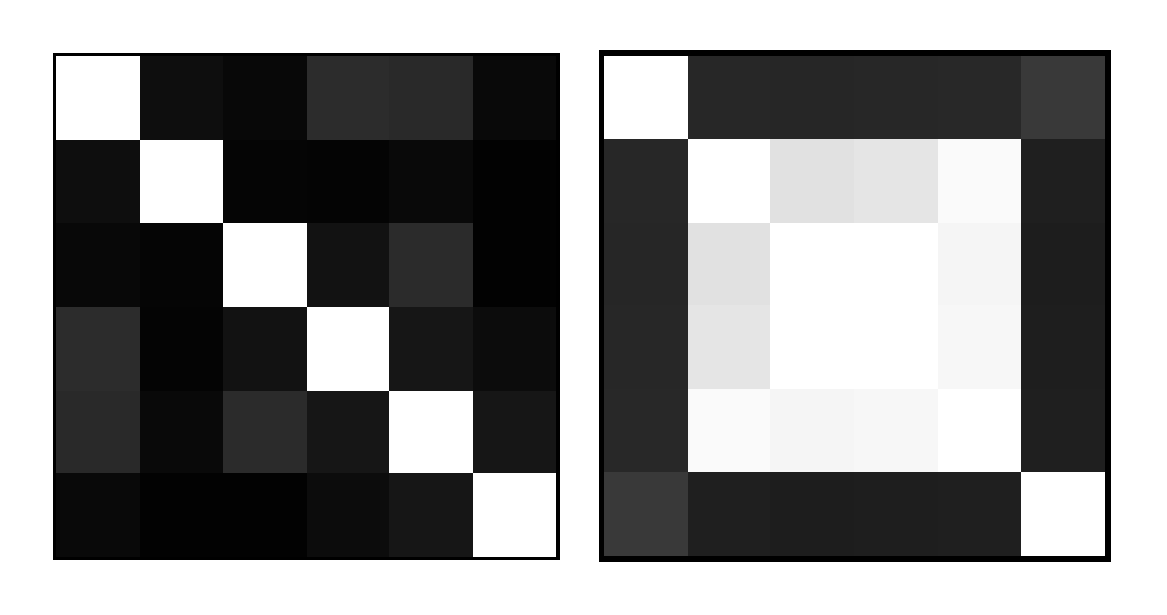
\includegraphics[width=0.8\textwidth]{images/faceCorrCompare.eps}
    \caption{Correlation matrix from learned representations. The left figure is for model C, and the right figure is for model D}
    \label{fig:FacesamplesModel3}
\end{figure}






\subsection{Norb dataset}

\begin{figure}
\centering
    \begin{subfigure}[b]{0.5\textwidth}
    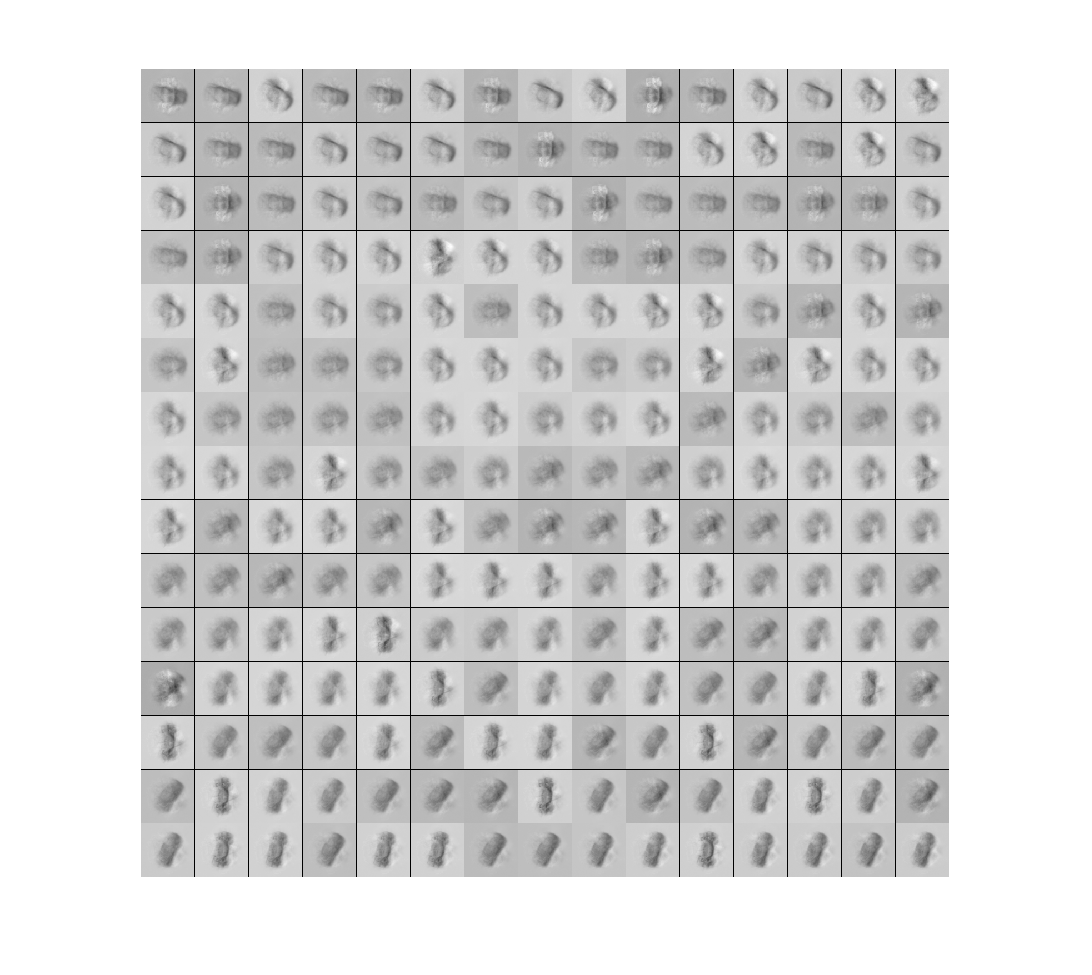
\includegraphics[width=\textwidth]{images/norbNWblock1sample.eps}
    \vspace{-2\baselineskip}
    \caption{Block 1 (2 hidden unit)}
    \end{subfigure}
	\begin{subfigure}[b]{0.5\textwidth}
    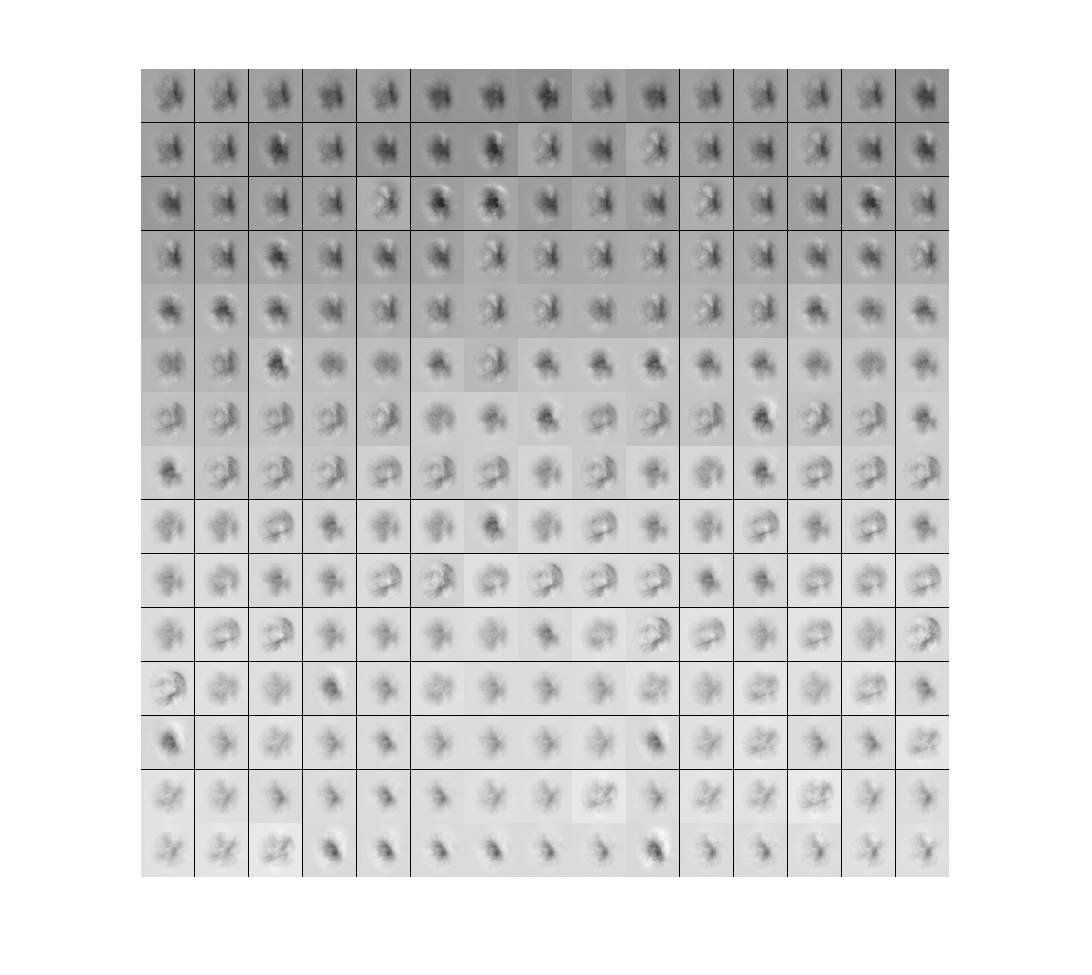
\includegraphics[width=\textwidth]{images/norbNWblock2sample.eps}
    \vspace{-2\baselineskip}
    \caption{Block 2 (2 hidden units)}
    \end{subfigure}
    \begin{subfigure}[b]{0.5\textwidth}
    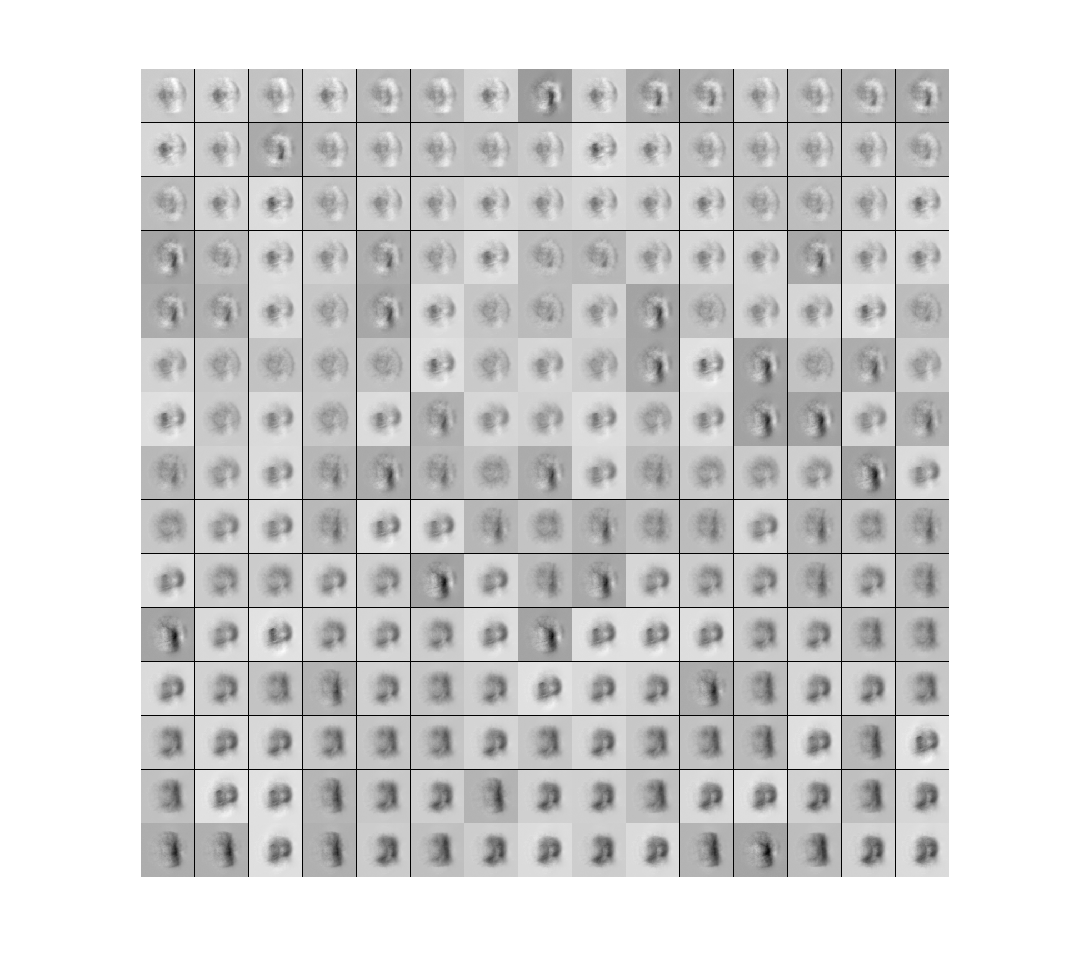
\includegraphics[width=\textwidth]{images/norbNWblock3sample.eps}
    \vspace{-2\baselineskip}
    \caption{Block 3 (2 hidden unit)}
    \end{subfigure}
    \caption{Generated face samples from \textbf{model C}. Block 1 means that we sample for block 1 and fixed others (with mean), and so on.}\label{fig:animals}
    \label{fig:norbsamples}
\end{figure}

In order to better understand the performance of our models. We also evaluate them on more complex datasets, which has three factors of variation. We use $6$ hidden units and we set the number of blocks to $3$. The Figure~\ref{fig:norbsamples} shows the generated samples from Model C. We can easily see that the block 1 encodes orientation, block 2 encodes the brightness and block 3 encodes the identity. 
 